\documentclass[10pt]{article}
\usepackage[backend=bibtex,style=numeric]{biblatex}
\usepackage{enumitem}
\usepackage{graphicx}
\usepackage{caption}
\usepackage{subcaption}
\usepackage{fullpage}

\addbibresource{refs}

\title{Extracting Application and Menu Events from UI Tutorial Videos}
\author{Daniel Seita \& Andrew Head}

\begin{document}

\maketitle

\section{Introduction}

In this project, we present two main contributions. First, we show that a standard neural network
following the AlexNet architecture with minimal tweaking can accurately recognize frames belonging
to a class of videos.  Second, we present a pipeline for detecting menus within a video frame
sequence. We then discuss how these two stages might be combined to enhance the process of
extracting information from videos.

\subsection{Motivation}

The proliferation of video tutorials on using different software raises new research questions on
how to improve users' ability to learn from them~\cite{matejka_ambient_2011,
pongnumkul_pause-and-play_2011}.  One strength of video tutorials is that users can directly observe
expert use, which can serve as a strong learning aid. Grossman \& Fitzmaurice showed that short,
10-25 second contextually-related videos were more effective to help users accomplish tasks than
traditional text-based tutorials~\cite{grossman_toolclips_2010}.  Unfortunately, video tutorials
have drawbacks. Navigation issues could lead to misunderstanding of content, and users may not be
able to keep up with the pace of instruction. Researchers working with longer, 2-3 minute
task-oriented tutorials found that users performed better with text tutorials than videos because
users could not work at the same pace as the video~\cite{grabler_generating_2009}.

In general, research on instructional videos point shows a need to segment videos to emphasize
certain steps. One way to automatically segment existing videos is to develop techniques for
detecting locations of certain menu actions in videos. Our goal, therefore, is to do this by
utilizing computer vision techniques.


\subsection{Related Work}

By examining pixels, many have succeeded at reverse engineering user interfaces and interactions
with purely visual information, independent of any knowledge of underlying application
implementations. For instance, Sikuli~\cite{yeh_sikuli_2009} uses computer vision to identify GUI
elements from screen captures, using template matching for small UI elements and voting based on
invariant local features for large elements. Sikuli allows users to search for documentation related
to screenshots of UI elements, and to script GUI tasks using visual cues.

Pause-and-Play extends the template matching approach of Sikuli to detect tool-selection UI events
in compressed, low-resolution video tutorials.  The system takes a tool palette template and tool
icons as input, producing metadata file of tool changes with timecodes.  With template matching at
multiple resolutions, detection is invariant to recording resolution and some camera
effects~\cite{pongnumkul_pause-and-play_2011}.


% Can cite these but we need more space for actual content: ~\cite{dixon_content_2011}~\cite{dixon_general-purpose_2012}.
Prefab identifies GUI elements with GUI specific visual features~\cite{dixon_prefab_2010}, which
enables overlay of advanced interactions on existing interfaces.  Prefab identifies interface
elements using a library of prototypes.  This uses two strategies: exact matches of prototype pixels
against an image, and modelining the prototype background and differencing pixel in an image to
identify foreground interface elements.  Prefab generalizes from example images to models which
contain parts like exact pixel features, or regions or areas of variable size or repeating patterns.
It organizes the entire interface into a hierarchy.

Waken contributes to this space by discovering cursor shapes, clicking actions, icons, tooltips and
menus, all by examining the difference between frames of UI video.  They do this by making
assumptions about how the image of icons change during hover and press actions.  Detection of the
cursor and icons in later frames is performed by template matching~\cite{banovic_waken_2012}.  We
rely on techniques similar to those in Waken to establish when menus have been activated and menu
items selected.


\section{Video Classification}\label{sec:daniel}

As a first step in the information extraction pipeline, we consider the following classification
question: given a video tutorial, what application is it about? As an extra challenge, we will only
assume we have access to the raw frames, and not other meta data such as the video title, etc.
(Knowing that a video is called ``Eclipse Tutorial \#5'' would make the task too easy.) The
rationale for analyzing this classification problem is that if we know the application that forms
the basis of the video tutorial, then we can further specialize information extraction procedures.
For instance, we might develop templates for matching Eclipse menu items, which would be deployed
only if we are reasonably confident that a video tutorial is actually about Eclipse. Furthermore, if
a video contains multiple applications (e.g., a video might contain Excel, Powerpoint, and other
Microsoft Office products), we might be able to segment the video based on application type, which
relates to the need to partition videos.

\begin{figure}[t]
\centering
  \begin{minipage}{.48\textwidth}
  \centering
  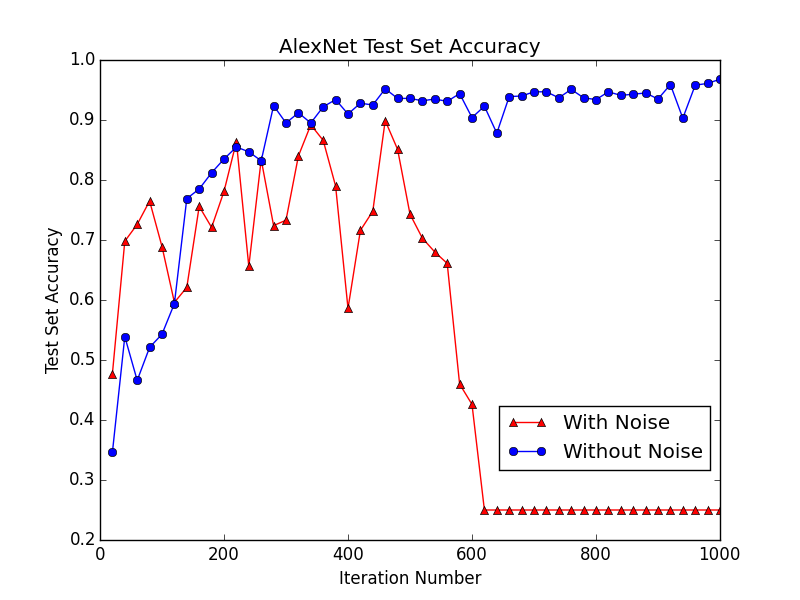
\includegraphics[width=1\linewidth]{AlexNet_Accuracy1000}
  \caption{AlexNet accuracy results of two networks trained on two image datasets.}
  \label{fig:alex_net}
  \end{minipage}\hfill
  \begin{minipage}{.48\textwidth}
  \centering
  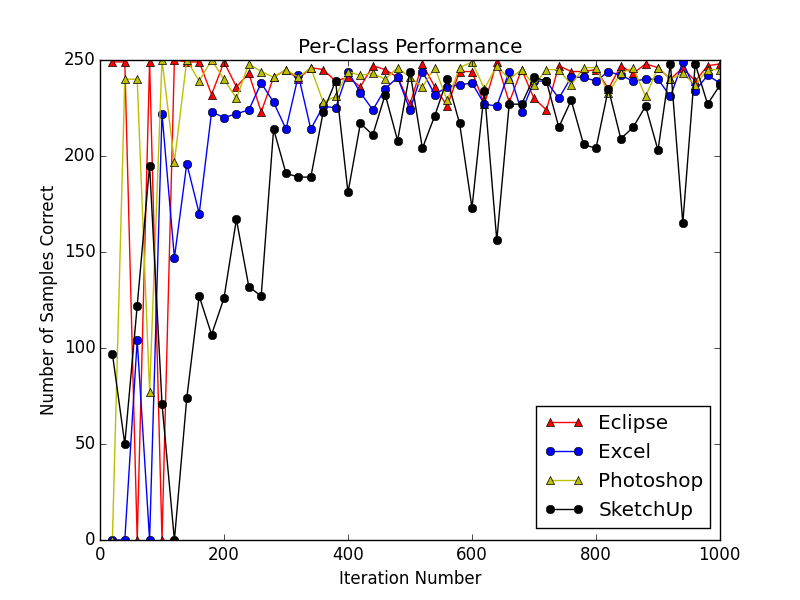
\includegraphics[width=1\linewidth]{PerClassPerformance1000}
  \caption{AlexNet per-class accuracy results for the network trained on ``no noise'' data.}
  \label{fig:per_class}
  \end{minipage}
\end{figure}

To collect training data, we used the open source \texttt{youtube-dl} software to download videos
from YouTube into mp4 format. We restricted our focus to videos about Eclipse, Excel, Photoshop, and
SketchUp, and we extracted from playlists to maintain consistency among the four classes. Most
videos were four to fifteen minutes long.  Then, we used the open source \texttt{ffmpeg} software to
extract one frame per second from each video, which resulted in a set of about 110240 JPG images,
roughly evenly split among the four classes. We randomly divided this into training, validation, and
testing sets, with 52000 training images (13000 per class), 8000 validation images (2000 per class),
and 1000 testing images (250 per class). All images were resized to $256\times 256$ pixels.

We observed that many of the videos we found had specialized beginning and ending scenes that
created frames that were different from what we would expect for those videos. For instance, the
SketchUp videos we found had a lengthy 10-15 second introductory scene that was the same for all
videos, but was not very similar to the various scenes inside the actual tutorial portion of the
videos. Thus, we created two datasets: one with all the frames we extracted, and one with the
\emph{first and last ten frames removed} for each video. Since we had one frame per second, this was
equivalent to ``cropping'' each video by ten seconds on both sides. This cropped dataset, which also
included cropped validation and testing frames, was termed the ``no noise'' data.

To train our network, we used CAFFE's pre-provided AlexNet architecture, but increased the momentum
from 0.9 to 0.99 and decreased the base learning rate from 0.01 to 0.001. We had fairly small batch
size of 32 images, so our updates are relatively noisy. We ran training for 1000 iterations on both
datasets and saved every 20th architecture for testing purposes.

Figure~\ref{fig:alex_net} shows our accuracy results for the two AlexNet networks we trained on the
test set of 1000 images. One can see that the architecture trained on all the data performed
inconsistently on its testing data, and its accuracy eventually leveled off at 25 percent since it
always guessed that frames belonged to SketchUp videos. In contrast, the architecture trained and
tested on ``noiseless'' data performed about as good as we could have hoped for, with accuracy
peaking at 96.1 percent after 1000 iterations.

We also decided to investigate per-class accuracy results to see if certain types of video frames
were harder to learn than others. Figure~\ref{fig:per_class} shows our per-class accuracy results
for the ``no noise'' AlexNet network. For the first few iterations, accuracy varies wildly among the
classes since it is not uncommon for the network to always pick one class. After that, it seems
clear that the SketchUp videos are the hardest to learn since the black curve regularly shows worse
accuracy results than the others. Fortunately, by the time we reach about 500 iterations, our
network can correctly classify the vast majority of images across all four classes.

We then investigated the 96 filters for the first layer of the AlexNet architecture, each of which
has dimension $55\times 55$. Figures~\ref{fig:filters_all} and~\ref{fig:filters_nonoise} show
visualizations for the two architectures taken after 1000 iterations of training. There are some
interesting patterns present, such as straight lines and rough, curved shapes.

\begin{figure}[t]
\centering
  \begin{minipage}{.4\textwidth}
  \centering
  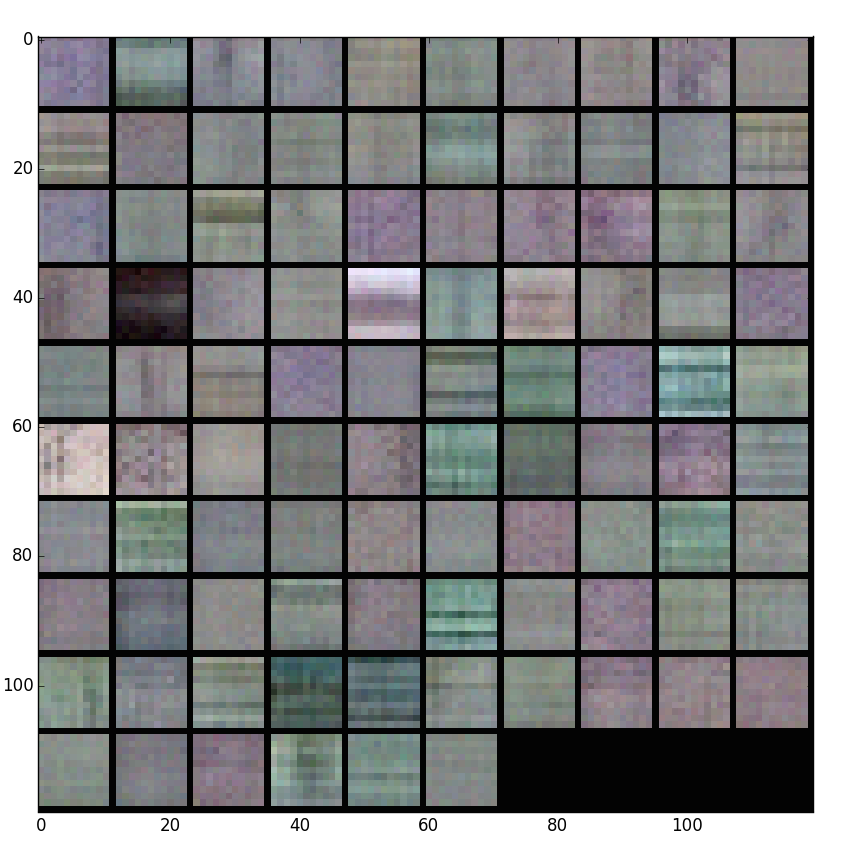
\includegraphics[width=1\linewidth]{Filters_All1000}
  \caption{Visualization of filters from the network trained on all our image data.}
  \label{fig:filters_all}
  \end{minipage}\hfill
  \begin{minipage}{.4\textwidth}
  \centering
  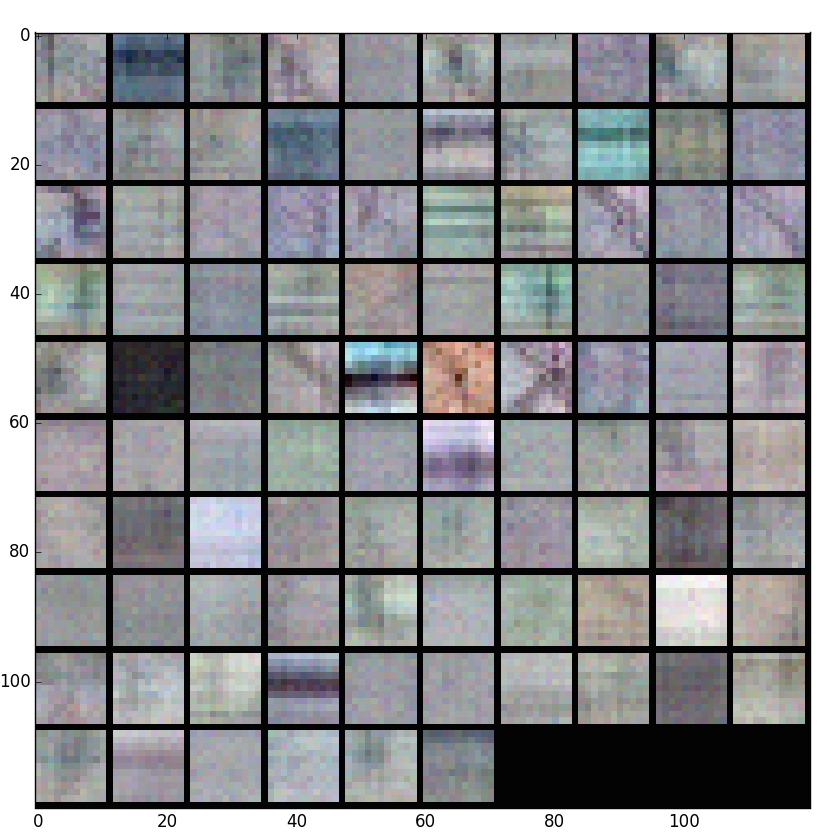
\includegraphics[width=1\linewidth]{Filters_NoNoise1000}
  \caption{Visualization of filters from the network trained on ``no noise'' image data.}
  \label{fig:filters_nonoise}
  \end{minipage}
\end{figure}

Finally, we performed a brief, informal experiment where we applied the neural network to videos that
were not part of our training or testing data. We chose one video for each of the four classes by
searching on Google Video ``X tutorial'' where ``X'' was replaced by one of the four video names.
The first video that was between 5 and 20 minutes long, and that was not already part of our
training/testing data, was selected. We extracted one frame per second for the four videos, and
deleted the first ten and final ten frames from consideration.

To classify the frames, we applied our AlexNet neural network trained on the ``noiseless'' data
after 1000 iterations. To describe the output, we use ``splits'' where $(a,b,c,d)$ indicates that
$a, b, c,$ and $d$ frames were classified as Eclipse, Excel, Photoshop, and SketchUp, respectively.
The splits were as follows: the Eclipse video had $(319,0,79,0)$, the Excel video had
$(610,0,71,7)$, the Photoshop had $(1,6,416,69)$, and the SketchUp had $(9,2,233,804)$. Clearly, for
the Eclipse, Photoshop, and SketchUp videos, the classifer was able to assign the vast majority of
frames to the correct class. If we were using this as part of an overall data mining pipeline, our
classifier would assign the video according to the most-assigned class, so three videos would be
classified correctly.

The Excel output is interesting, because our network thought most of the frames belonged to Eclipse
videos. A brief look at the video indicated that it had an introductory scene that took up ninety
seconds (and we only deleted the first 10 frames) and that it was about a newer version of Excel
(2013) than the ones that were trained in our network (2007). Still, it is unfortunate but shows
that we need to be able to provide a wider variety of training data.

\section{Locating Menus in a Frame Sequence}\label{andrew}

This will be Andrew's section.

Answer these questions:
\begin{enumerate}[noitemsep]
\item What is our dataset?
\item How did we construct/acquire it?
\item What's its size?
\item (optional) How will we improve it in the future?
\end{enumerate}

Here's a figure of our (edit: Andrew's) pipeline.  \textbf{Andrew: Add figure of pipeline.}

Here we (edit: Andrew) want to touch upon:
\begin{enumerate}[noitemsep]
\item How reliably can we classify UI events?
\item How long does it take for us to process one minute of video?  What are
the practical implications of this?
\item Some images that show recognition results for a few representative
screenshots of user interfaces.
\end{enumerate}


\section{Discussion and Conclusion}

TODO (combining the two because we don't have a lot of space!)

We freakin' rock.

\printbibliography

\end{document}
